\documentclass[10pt,letterpaper]{article}
\usepackage[utf8]{inputenc}
\usepackage[T1]{fontenc}
\usepackage{amsmath}
\usepackage{amsfonts}
\usepackage{amssymb}
\usepackage{graphicx}
\usepackage{cleveref}
\author{Mike Sutherland}y
\title{Homework 3}
\begin{document}
    \maketitle
    
    \section{Problem 1 - Lagrange Interpolation}
    First, we construct a function to generate Lagrange polynomials of a general order and for a general set of evaluated points.
    \begin{figure}[h]
        \centering
        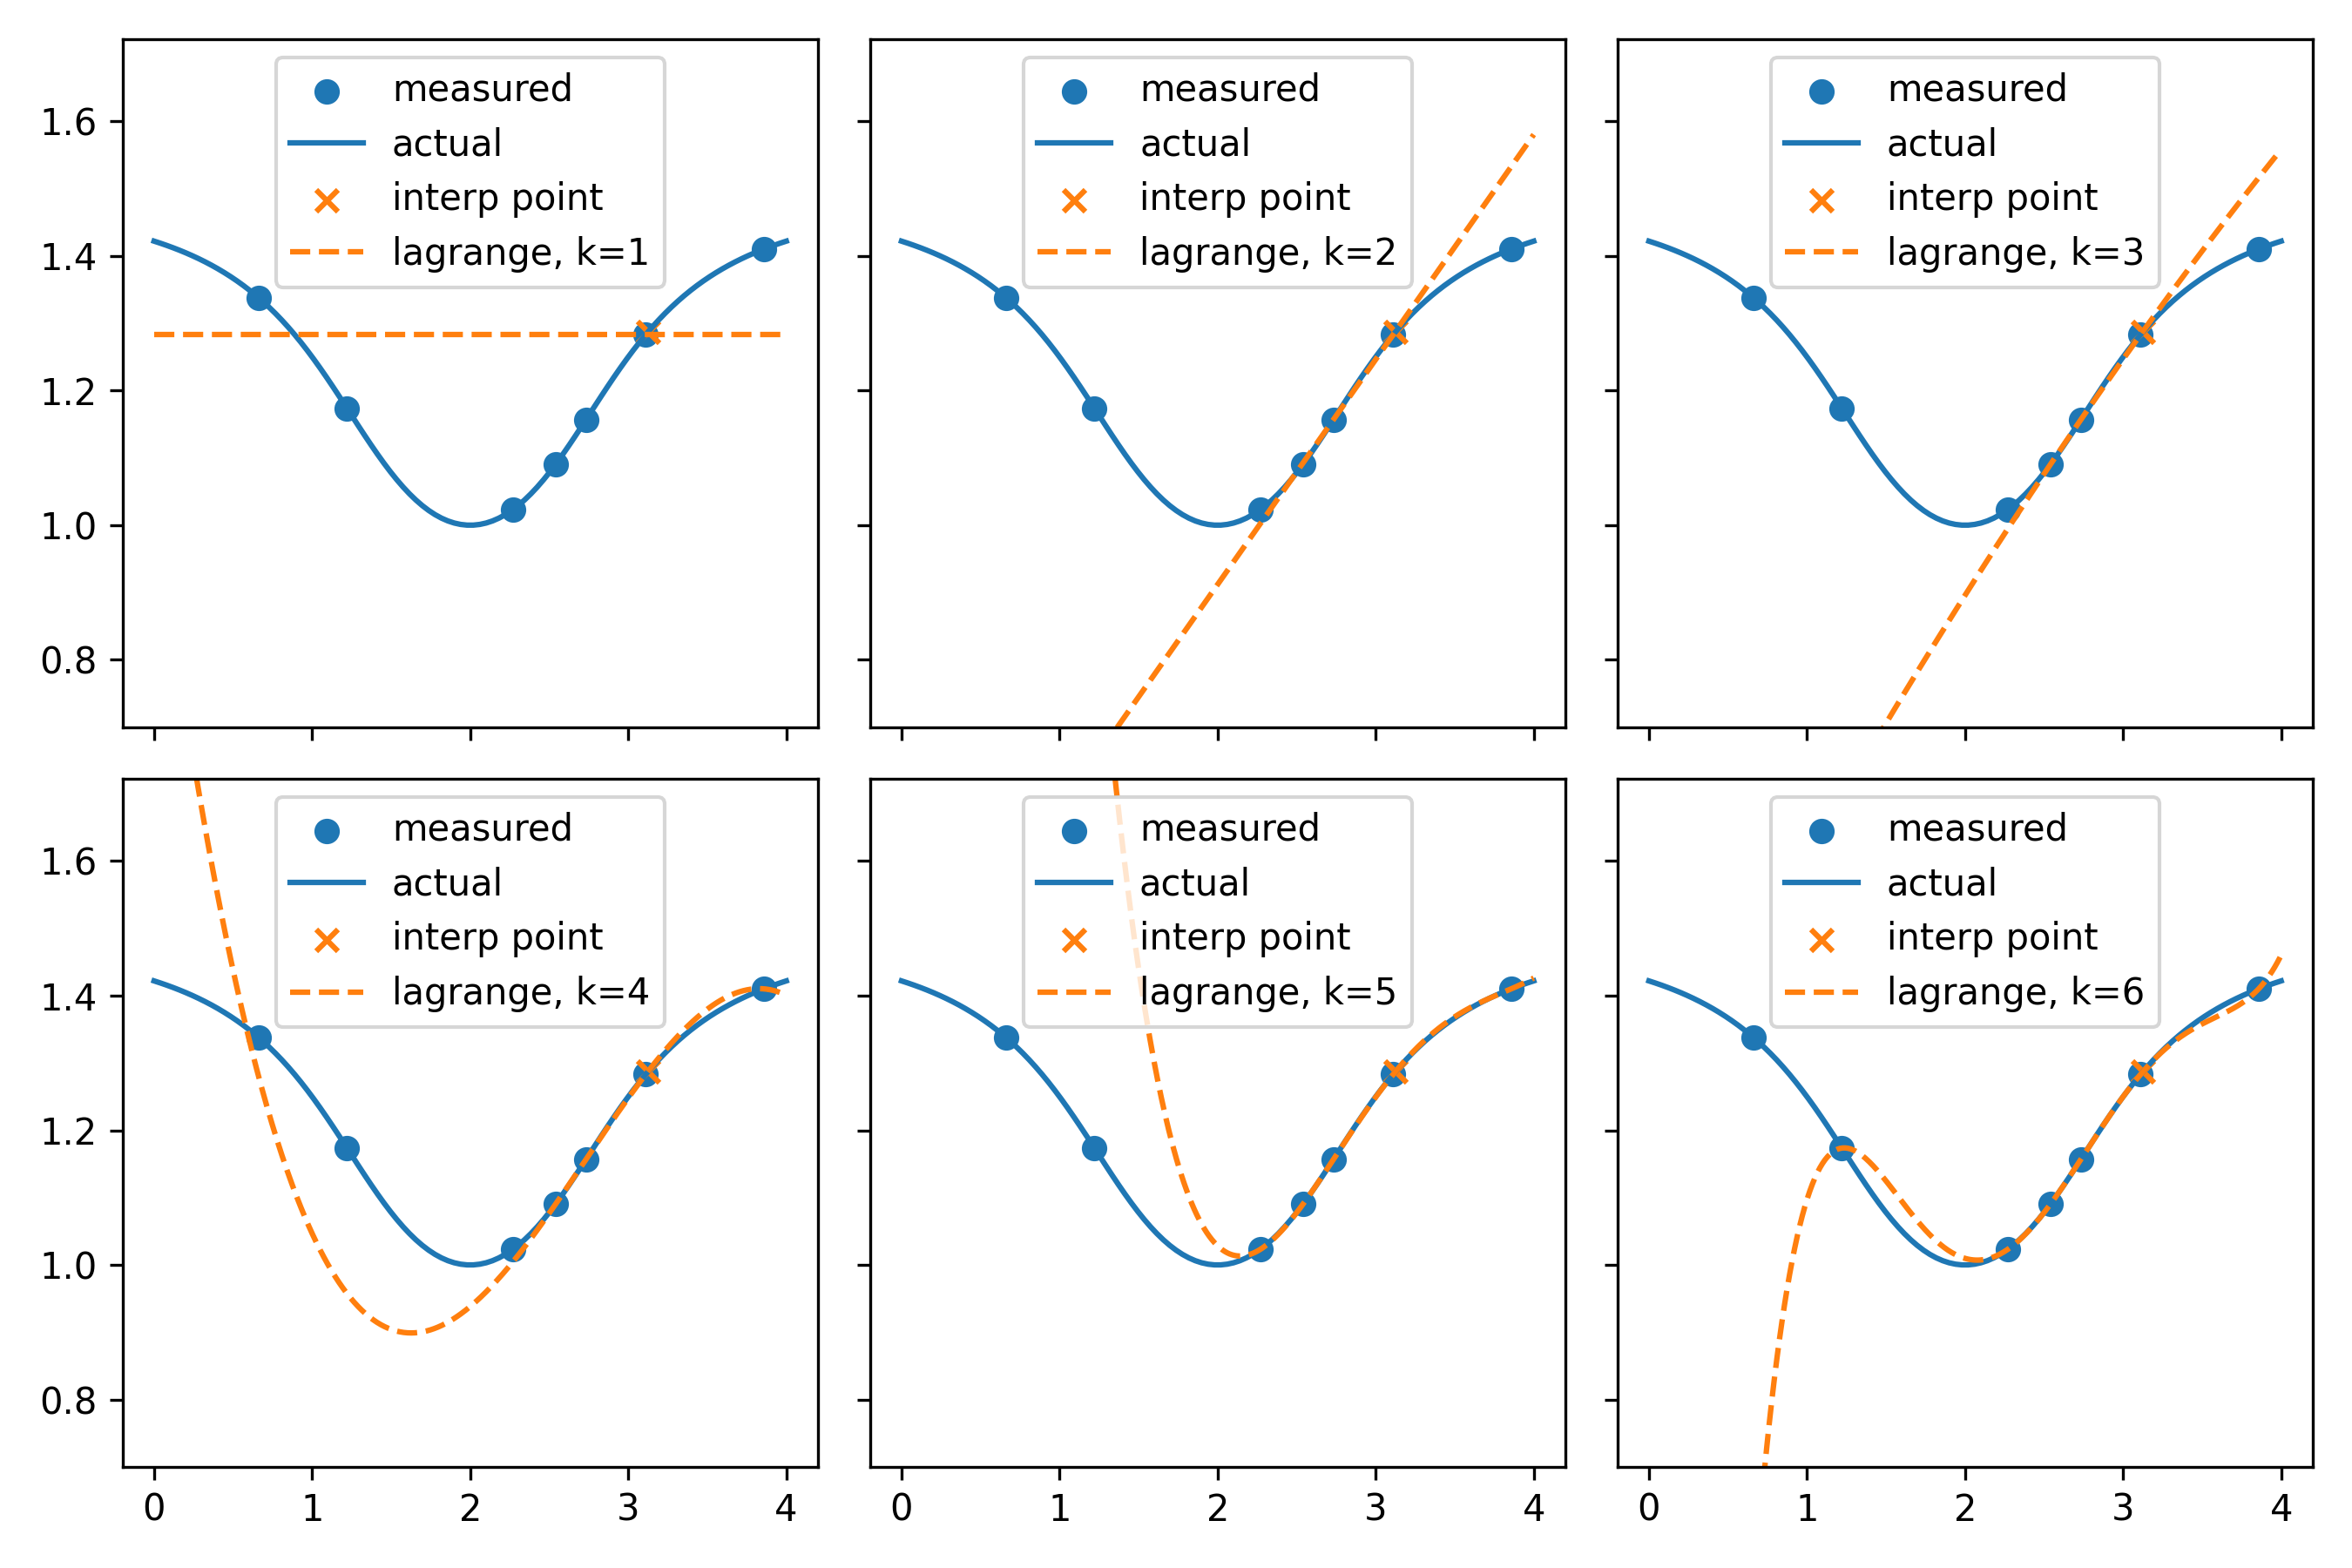
\includegraphics[width=1.0\linewidth]{../plots/lagrange.png}
        \caption{A series of lagrange plots of various order. The true function is the transcendental function $\arctan((x-2)^2)/\pi + 1$. We can see that as we add more points, the approximation becomes more accurate; however, there is also more overshoot.}
        \label{fig:lagrange}
    \end{figure}
    The results for this function on some test data is shown in \cref{fig:lagrange}. We can see the effect of increasing order on the accuracy of the approximation; with increased order, the approximation could become more accurate, but it also is subject to more extreme overshoot. We can also see how the order of the constructed polynomial affects the direction of extrapolation: the sign of extrapolated points changes with odd/even orders of lagrange polynomials.

    We turn to the example data of Problem 1.
    \begin{figure}[h]
        \centering
        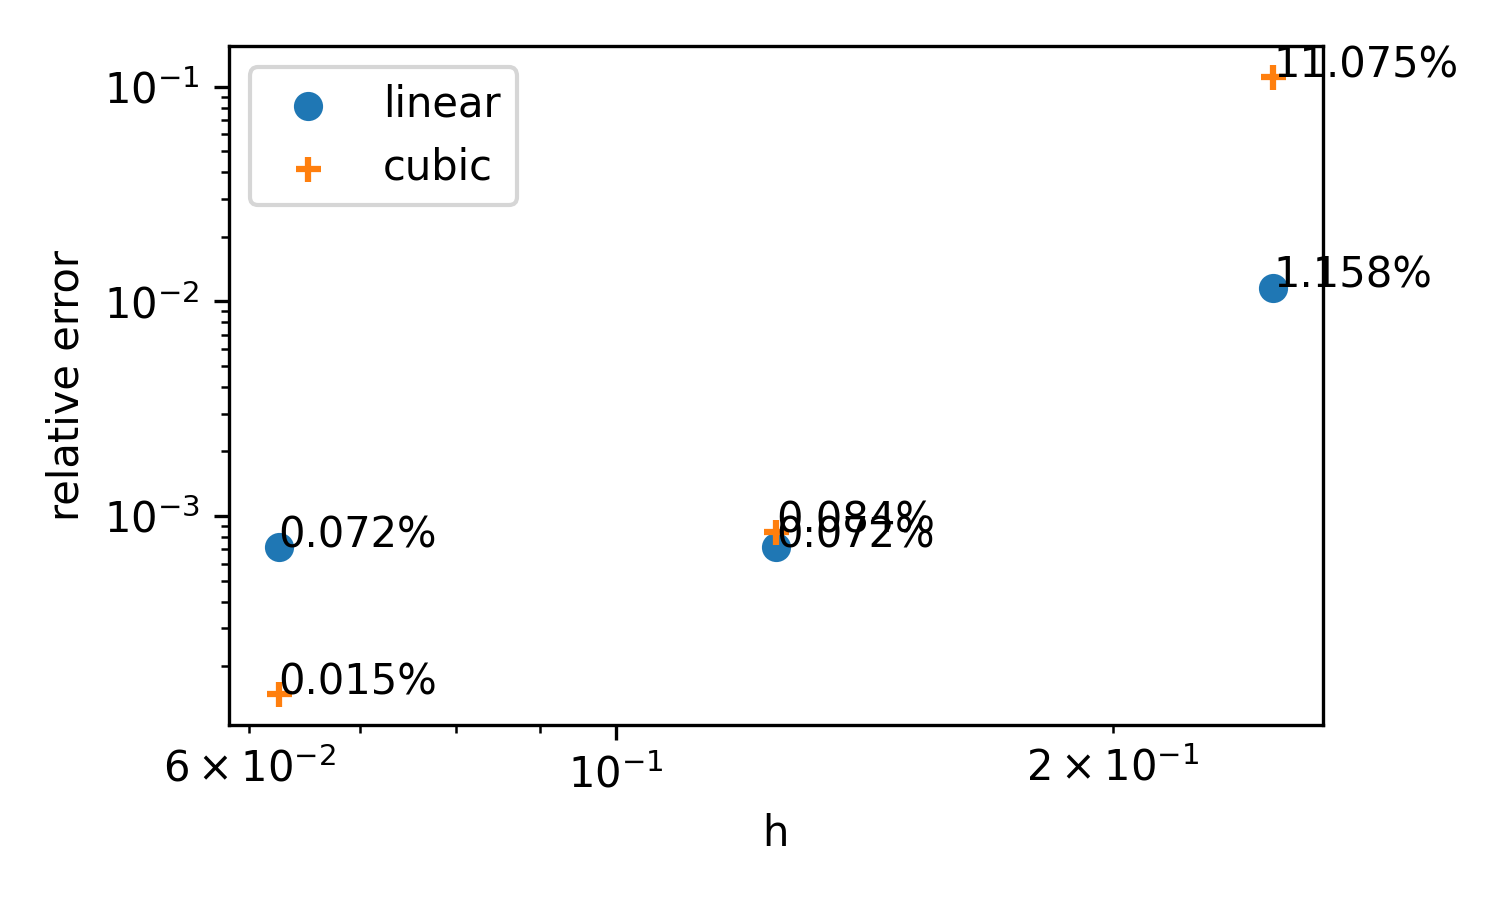
\includegraphics[width=0.9\linewidth]{../plots/lagrange_error.png}
        \caption{Lagrange interpolation of polynomials and their respective error. For small values of $h$, the error is smaller for the higher-order polynomial. However, for larger values of $h$, the error is smaller for the lower-order polynomial.}
        \label{fig:lagrange_error}
    \end{figure}
    We can see from \cref{fig:lagrange_error} the effect of the order of the polynomial on the error of the solution, as it relates to the step size of the sampled data. We can see how lower-order polynomials obtain worse interpolation for small step sizes, while higher-order polynomials obtain worse interpolation for large step sizes. As the order of the polynomial increases, the fluctuations in areas between data points become larger, due to the presence of higher-order terms.

    The optimal order of a Lagrange polynomial varies depending on the data being sampled. If the structure of the data is unkown before performing the interpolation, lower-order polynomials (usually, cubic) are used, because they often obtain a better fit than linear interpolation, while limiting the overshoot. For functions that are polynomials, a Lagrange polynomial of the same order as the original function will produce an exact fit of the data.

    Because of the overshoot issue with Lagrange polynomials, they are often not be suitable for noisy data. In those cases, it may be wise to either filter the data or use a different technique, like Gaussian Process Regression with a rational quadratic kernel.

    We also notice that Lagrange polynomial interpolation is not suitable for extrapolation, since the polynomial is unbounded.
    \subsection{Problem 2}
    [to do]
    \section{Problem 3 - Integration} 
   To solve Problem 2, we created a python program that computes the integral of a given function over an interval using the Trapezoid rule. 

    \begin{figure}
        \centering
        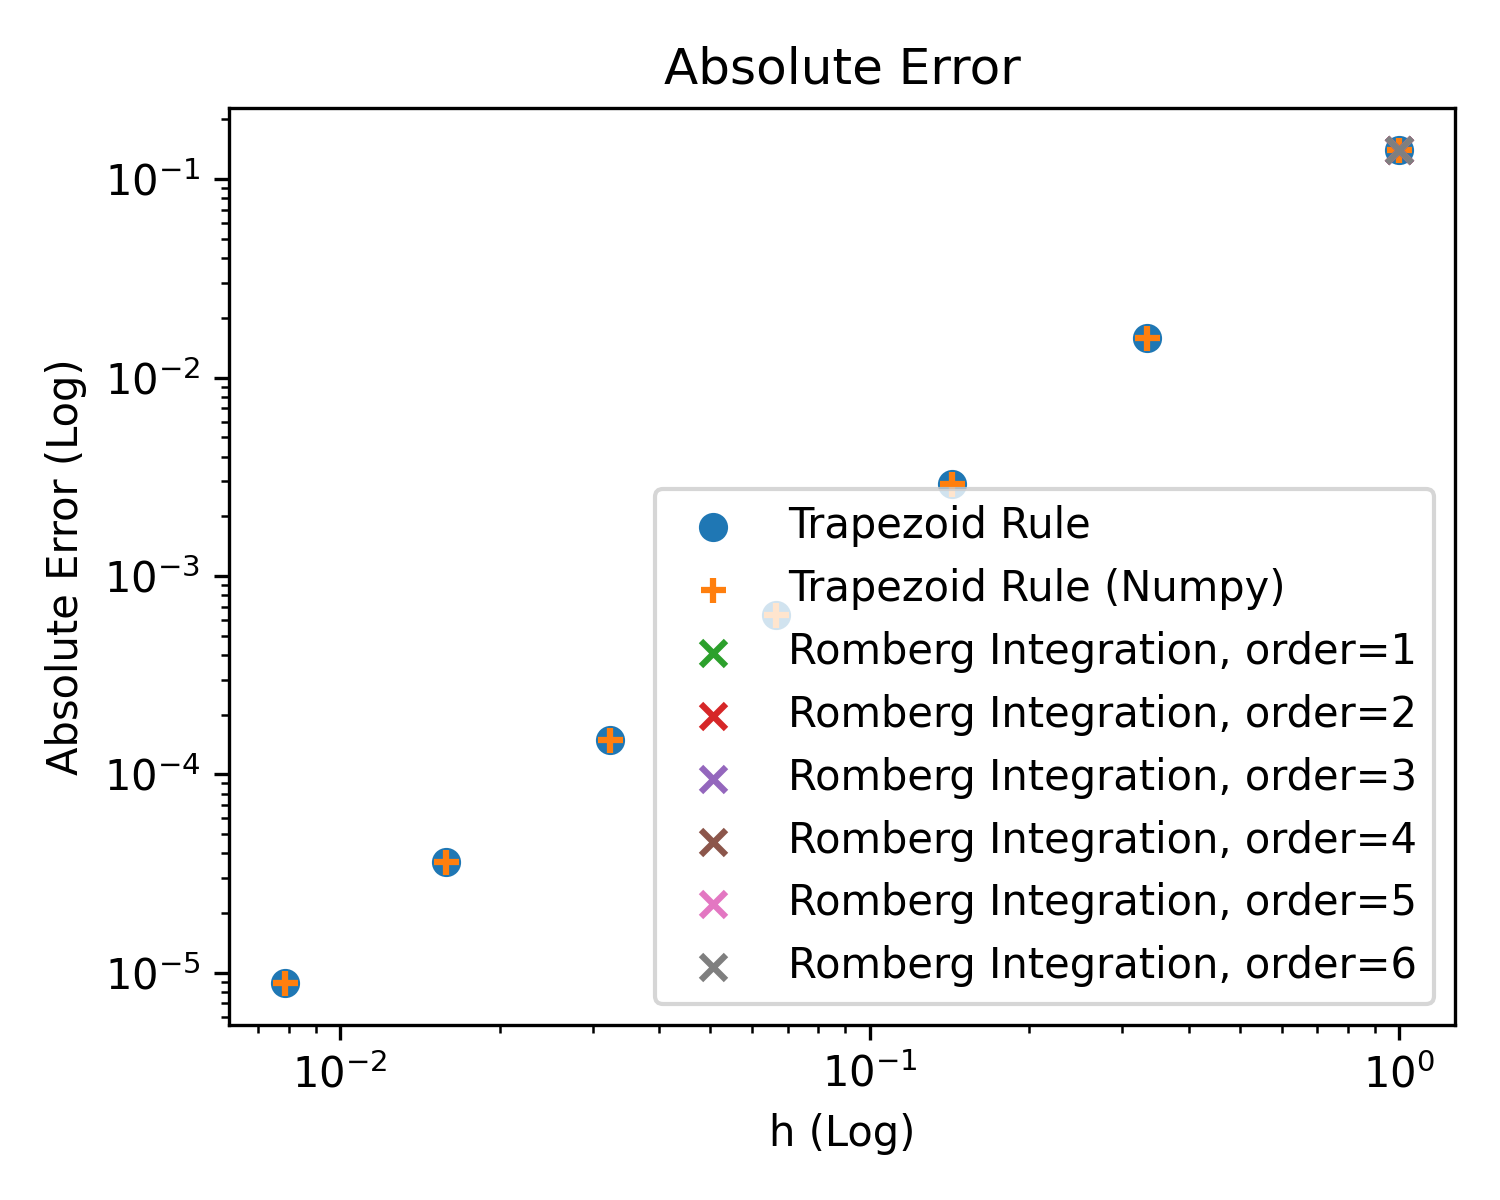
\includegraphics[width=0.6\linewidth]{../plots/integration.png}
        \caption{Log-Log plot of the absolute error vs the step size, as compared with the analytic solution of a known integral. We can see that as the step size decreases, the error decreases in turn, until the step size is so small that round-off error becomes an issue.}
        \label{fig:integration_err}
    \end{figure}
    The trapezoid rule computes the integral of a function by summing the area of trapezoids evaluated at points along a function. If a smaller step size is used, more linear segments of the original function are evaluated, which reduces the error. The relationship between error and step size is order $\mathcal{O}(h)$ because of this linear relationship. This is effect is visible in \cref{fig:integration_err}.

    \begin{figure}
        \centering
        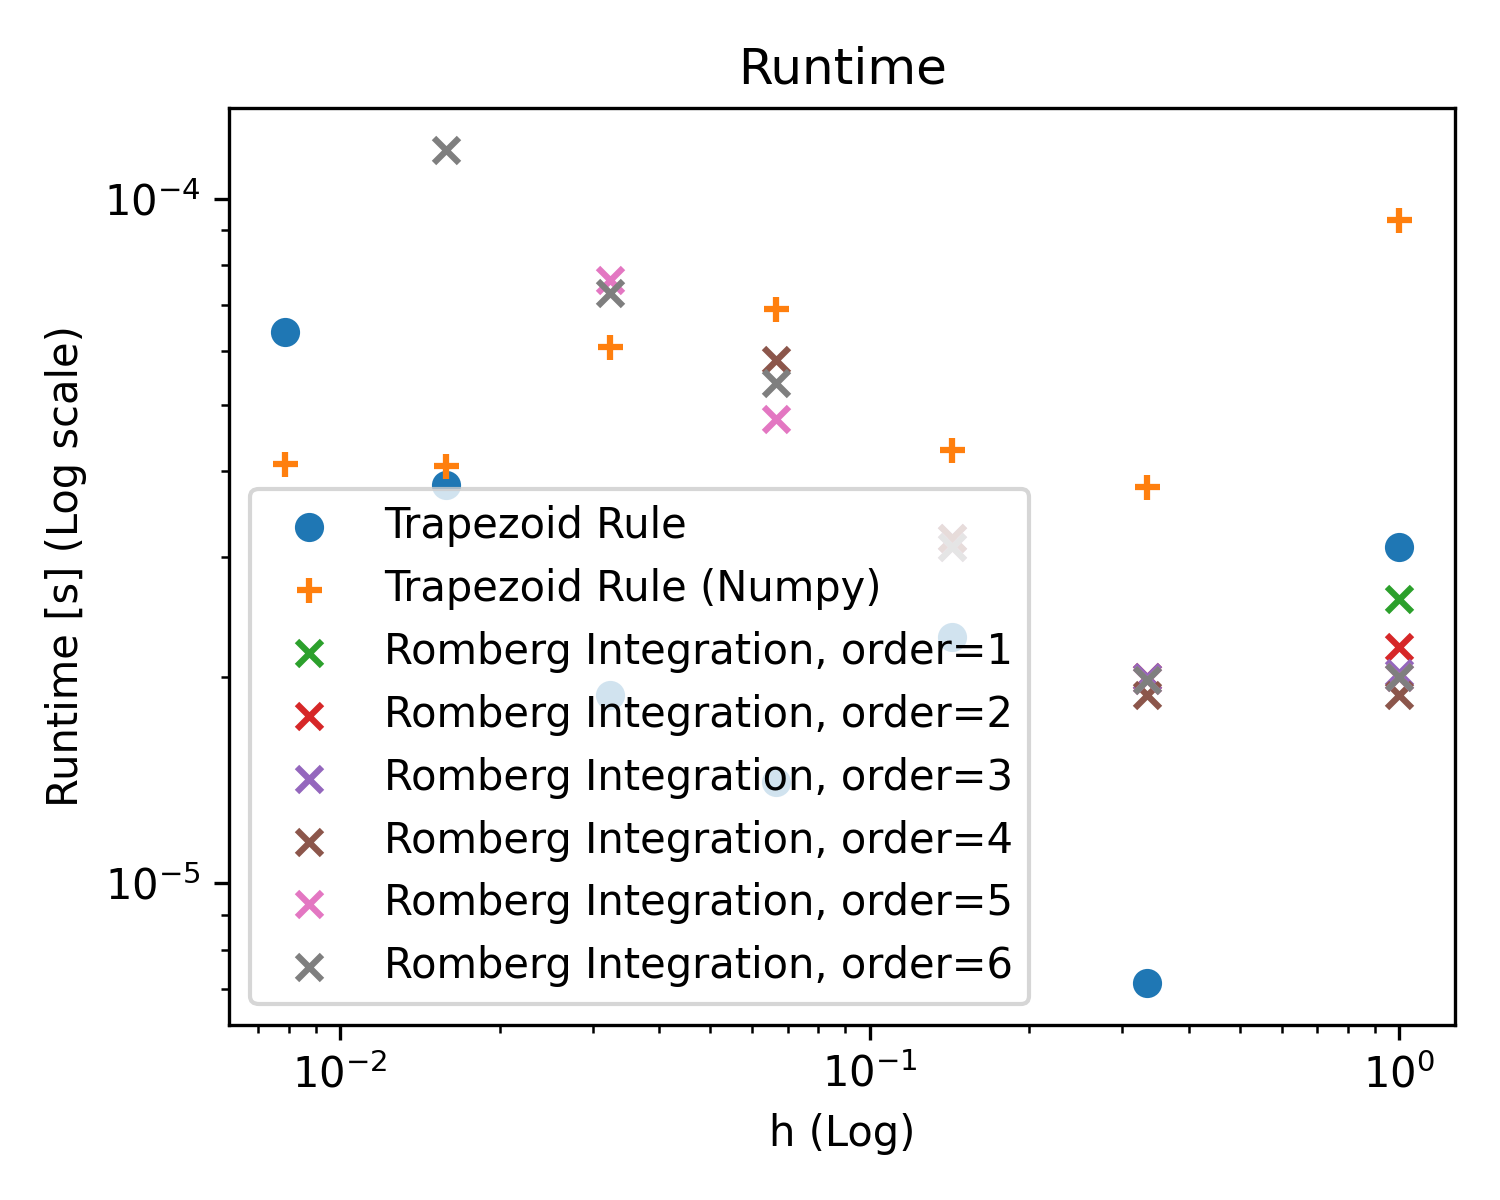
\includegraphics[width=0.7\linewidth]{../plots/integration_runtime.png}
        \caption{Log-Log Runtime of a naive trapezoid rule, \texttt{np.trapz}, and a Romberg integration, vs. $h$. We can see that as $h$ decreases, runtime increases. The relationship is $\mathcal{O}(h)$. The naive python implementations have a higher overhead than their numpy variants.}
        \label{fig:integration_runtime}
    \end{figure}

    We evaluate the runtime in \cref{fig:integration_runtime}. We can see that the runtime increases linearly with a decrease in step size.

    Romberg integration has a runtime comparable to naive trapezoid integration; its benefit is that as the algorithm runs, the evaluated integral is visible to the algorithm, which makes it useful when the programmer needs to specify expected error ahead of time, without knowing ahead of time what step size results in that expected error.
    \section{Problem 4 - Differentiation}
    We created a program which differentiates a given function using a 2nd order and 4th order central difference scheme.

    \begin{figure}
        \centering
        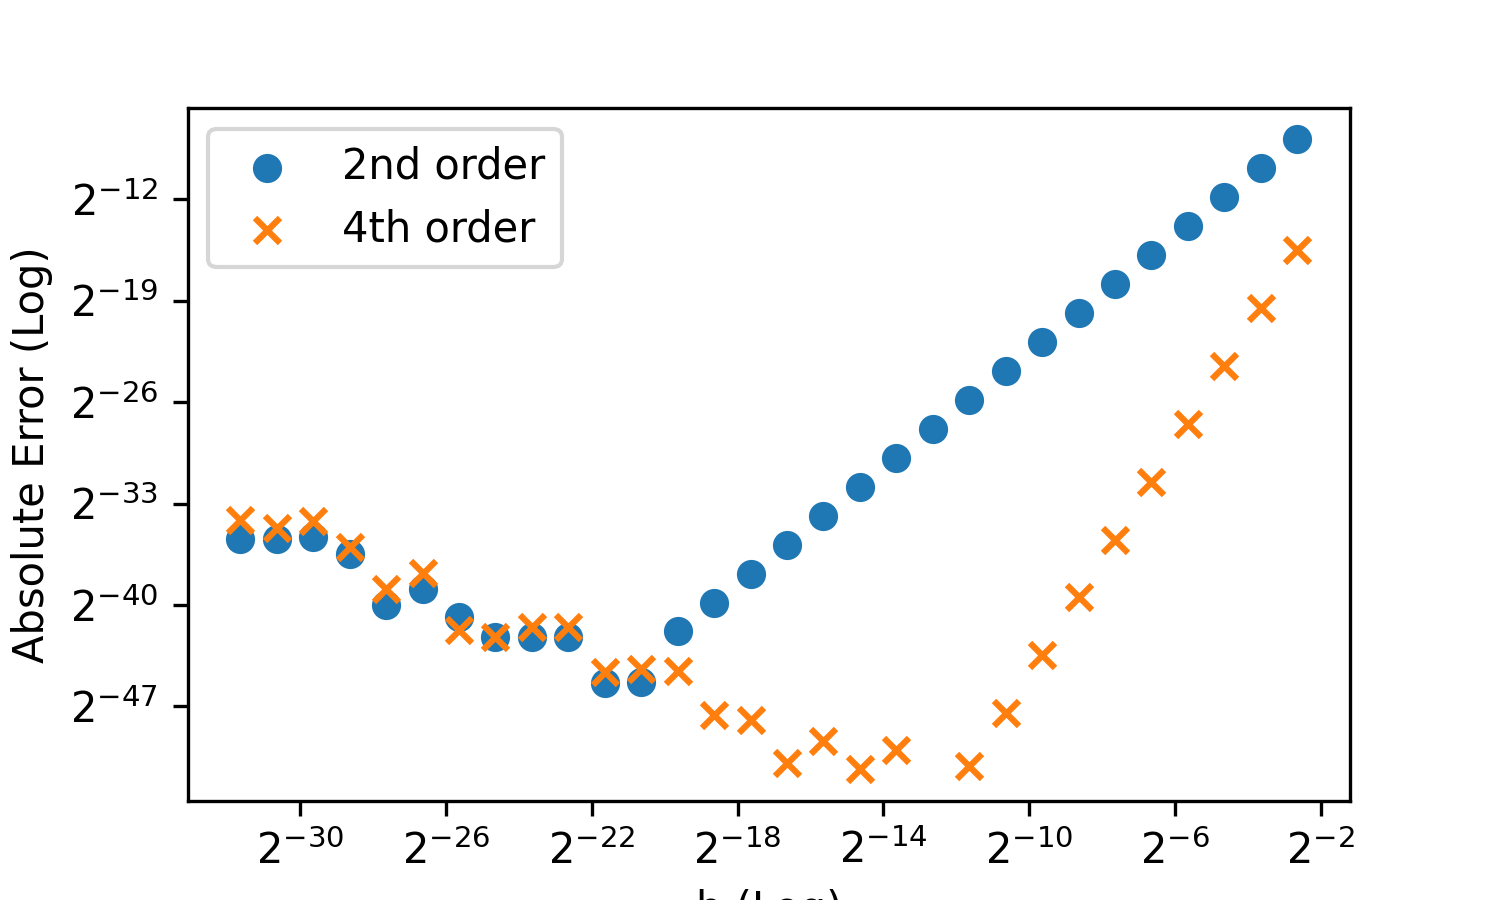
\includegraphics[width=0.7\linewidth]{../plots/derivs.png}
        \caption{Differentiation of a function using a 2nd order and 4th order central difference scheme. The 2nd order central difference scheme is less accurate than the 4th order central difference scheme. The limit of numerical precision is visible for both schemes.}
        \label{fig:diff_err}
    \end{figure}

    \Cref{fig:diff_err} shows the relationship between the step size and error of 2nd and 4th order numerical derivatives. The 4th order scheme is more accurate (its error is $\mathcal{O}(h^4)$) than the 2nd order scheme (its error is $\mathcal{O}(h^2)$). However, because of the additional multiplication of $h$ in the denominator of the 4th order scheme, it runs into the limits of numerical precision faster than the 2nd order scheme. Despite this, it is ultimately more accurate.
    \section{Problem 6 - Differentiation}
    \textit{Explain how you would construct a 6th-order accurate central finite difference approximation for the first derivative on a uniform grid.}
    We begin with a general expression for the taylor series:
    \begin{equation}
        f(x_{i+1}) = f(x_i) + f'(x_i) h + \frac{1}{2} f''(x_i) h^2 \dots
    \end{equation}
    In general, this yields a series of derivative terms. For an nth order term, we begin the Taylor series at $f^{n}(x_i)$. We can then rearrange these terms to obtain a system of equations:
    \begin{equation}
        f′(xi) = \frac{f(x_{i+1}) - f(x_{i+1})}{h}\\
        f''(xi) = \frac{f(x_{i+2}) - 2f(x_{i+1}) + f(x_{i})}{h^2}\\
        f'''(xi) = \frac{f(x_{i+2}) - 2f(x_{i+1}) + 2f(x_{i-1}) - f(x_{i-2})}{h^3}
    \end{equation}
    From the coefficients of these terms, we can construct a matrix and multiply to solve for the derivatives. We then evaluate the derivatives up to order $k+1$, plug them into the original Taylor series (of order $k+1$), and rearrange to solve for the derivative of the original function. The equations in this example were 2nd-order accurate, but the accuracy can be increased by taking higher-order terms from the original Taylor series.
    
    Because a general formula for the Taylor series is possible, any order can be constructed.
\end{document}